

\Aufgabe{Spieler programmieren}{
\begin{minipage}[t]{0.5\textwidth}
\normalsize
\vspace{-11cm}
    Probiere nach jedem Schritt aus, was passiert, wenn du dein Spiel startest!
    \begin{enumerate}
        \item Programmiere die Klasse Spieler wie im Klassendiagramm
        vorgegeben. Programmiere getX() und getY() als Standard-Getter, lasse
        act() erstmal leer.
        \item Erstelle einen Konstruktor und setze dort die Koordinaten
        auf feste Werte und finde damit heraus, wie groß das
        Spielfeld ist. Hierfür musst du etwas herumprobieren.
        \item Notiere den Programmcode von getX() und getY() auf der
        nächsten Seite.
        \item Das Spielfeld führt die Methode act() seiner Spieler-Objekte
        ca. 25x pro Sekunde aus. Finde heraus, wie du damit ein
        Spieler-Objekt auf dem Spielfeld bewegen kannst.
        \item Wie kann man die Bewegungsgeschwindigkeit des Spiel-
        ers festlegen? Probiere deine Idee im Programm aus und
        ergänze das Klassendiagramm und den Programmcode auf
        der nächsten Seite.
        \item Wie kann man zu Beginn des Spiels die Startposition des
        Spielers (bei jedem neuen Objekt woanders) festlegen? Pro-
        biere auch das wieder aus und ergänze das Klassendia-
        gramm.
        \item Über den Toolbox-Ordner `Grafik: Objekte` kannst du in der Main 
        weitere geometrische Formen hinzufügen. Nutze das, um ein kleines 
        Spiel zu programmieren.
    \end{enumerate}
\end{minipage}
\hfill
\begin{minipage}[t]{0.47\textwidth}
\large
%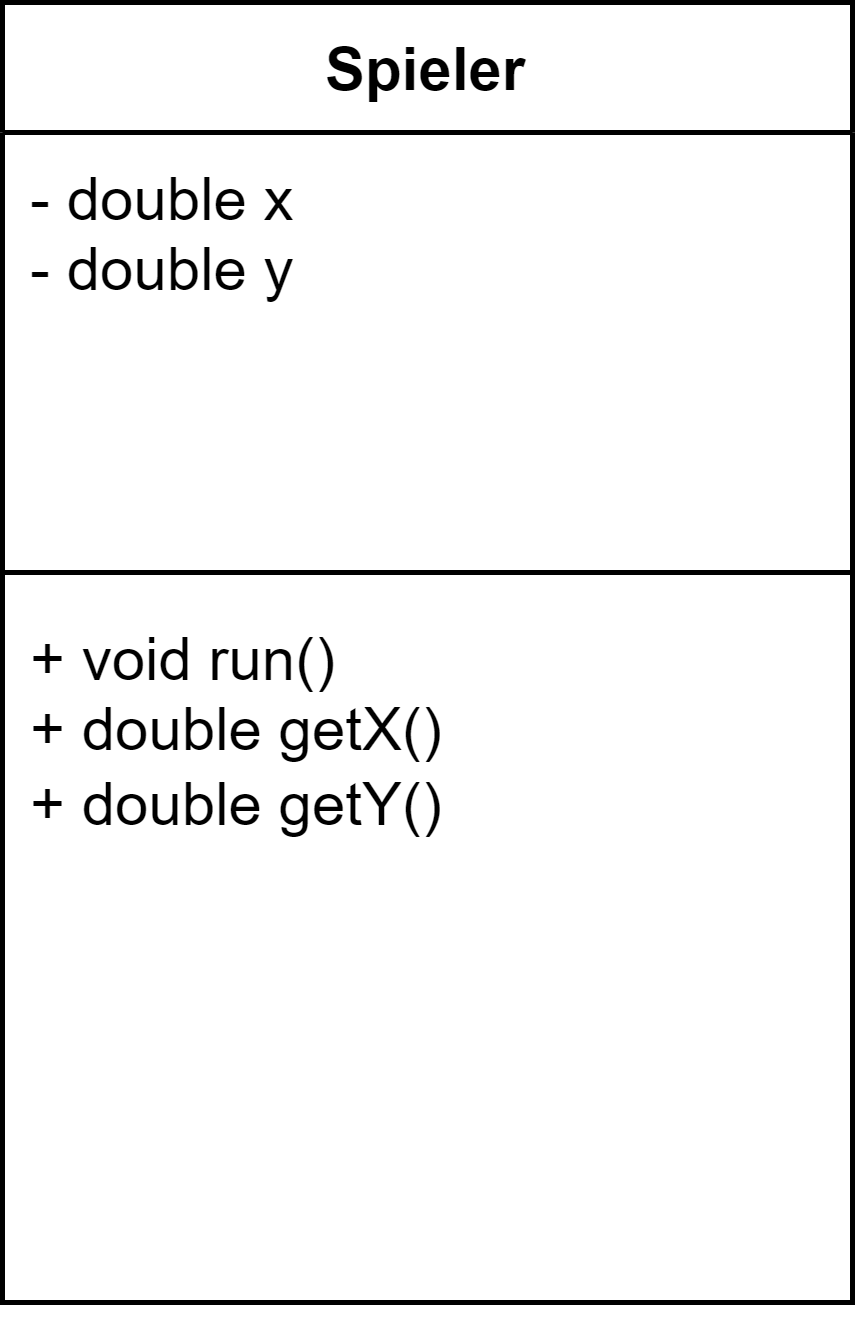
\includegraphics[width=0.9\linewidth]{_Aufgaben/BlocksAndJava/img/57_Klassendiagramm.png}
\begin{tikzpicture}
\begin{class}[text width=\linewidth]{Spieler}{0 ,0}
\attribute{- double x}
\attribute{- double y}
\attribute{}
\attribute{}
\attribute{}
\attribute{}
\attribute{}
\operation{+ void act()}
\operation{+ double getX()}
\operation{+ double getY()}
\operation{}
\operation{}
\operation{}
\operation{}
\operation{}
\operation{}
\operation{}
\operation{}
\operation{}
\operation{}
\operation{}
\end{class}
\end{tikzpicture}
\end{minipage}
}

\pagebreak

\large
\begin{lstlisting}
public class Spieler {
    private double x;
    private double y;

    (*@\LoesungLuecke{private double speedX;}{10cm}@*)

    (*@\LoesungLuecke{private double speedY;}{10cm}@*)
    
    public double getX() {
    
        (*@\LoesungLuecke{return x;}{10cm}@*)
    }
    public double getY() {
    
        (*@\LoesungLuecke{return y;}{10cm}@*)
    }
    public void act() {
    
        (*@\LoesungLuecke{x += speedX;}{10cm}@*)
        
        (*@\LoesungLuecke{y += speedY;}{10cm}@*)
        
        (*@\LoesungLuecke{y += speedY;}{10cm}@*)
        
        (*@\LoesungLuecke{y += speedY;}{10cm}@*)
        
        (*@\LoesungLuecke{y += speedY;}{10cm}@*)
    }
    
    public void (*@\LoesungLuecke{setX(double wert}{10cm}@*) {
    
        (*@\LoesungLuecke{x = wert;}{10cm}@*)
    }
    
    public void (*@\LoesungLuecke{setY(double wert}{10cm}@*) {
    
        (*@\LoesungLuecke{y = wert;}{10cm}@*)
    }
    
    public (*@\LoesungLuecke{Spieler(double startX, double startY}{10cm}@*) {
    
        (*@\LoesungLuecke{x = wert;}{15cm}@*)
        
        (*@\LoesungLuecke{y = wert;}{15cm}@*)
    }
}
\end{lstlisting}